%\documentclass[Serif, 10pt, brown, handout]{beamer} % Disable overlays for handout format
%\documentclass[Serif, 10pt, brown, handout, notes]{beamer} % Disable overlays for handout format and print notes
\documentclass[Serif, 10pt, brown]{beamer}
\usepackage{booktabs,xcolor}
%\usepackage[svgnames,table]{xcolor}
%\usepackage[tableposition=above]{caption}
\usepackage{pifont}
\newcommand*\CHECK{\ding{51}}
\usepackage{array}
\newcolumntype{P}[1]{>{\centering\arraybackslash}p{#1}}
%
\usepackage{setspace,mathtools,amssymb,multirow,array,amsmath,tikz}
\usepackage[normalsize]{subfigure}
\usetikzlibrary{patterns}
\usetikzlibrary{automata,positioning,decorations.pathreplacing,decorations}

\usepackage{curves}
\usepackage{wasysym}
\usepackage{epsfig,epstopdf,graphicx}

\curvewarnfalse
%
\newtheorem{proposition}{Proposition}
\theoremstyle{example}
\newtheorem{theoremh}{Theorem}
\theoremstyle{plain}
\renewcommand{\textfraction}{0.01}
\renewcommand{\floatpagefraction}{0.99}
\newcommand{\ul}{\underline}
\newcounter{units}
%
\usepackage[round]{natbib}
 \bibpunct[, ]{(}{)}{,}{a}{}{,}%
 \def\bibfont{\small}%
 \def\bibsep{\smallskipamount}%
 \def\bibhang{24pt}%
 \def\newblock{\ }%
 \def\BIBand{and}%
%
\setbeamercovered{dynamic}
% Logo
\logo{
\includegraphics[width=0.5in,keepaspectratio]{iitb_logo.png}}
%
% Setup
\mode<presentation>
	{
\usetheme[right,currentsection, hideothersubsections]{UTD}
			\useoutertheme{sidebar} \useinnertheme[shadow]{rounded}
			\usecolortheme{whale} \usecolortheme{orchid}
			\usefonttheme[onlymath]{serif}
			\setbeamertemplate{footline}{\centerline{Slide \insertframenumber/\inserttotalframenumber}}
	}
%
% Title
\usebeamercolor[fg]{author in sidebar}
\title[{Image Compression}]{\sc Image Compression Project}
\author[\ul{Authors}]{{\bf Saksham Rathi, Kavya Gupta, Shravan Srinivasa Raghavan}\\ \hspace{-1cm} (22B1003) \hspace{0.7cm} (22B1053) \hspace{1.7cm} (22B1054)}
\institute[UTD]{\sc\small CS663: Digital Image Processing\\ Under Prof. Ajit Rajwade}
\date[UCI]{Indian Institute of Technology Bombay \\ Autumn 2024}
%
%Presentation
\begin{document}
\frame{\titlepage}
%
%
%Slides

%TOC

\begin{frame}
	\transblindsvertical
	\frametitle{Contents}
	\tableofcontents[hidesubsections]
\end{frame}
\note[itemize]{
\item Here's the overall structure of my talk today.
}


% Introduction
\section[Problem Statement]{Problem Statement}
% 
% \setbeamercolor{background canvas}{use=structure,bg=white}
% \setbeamercolor{background}{use=structure,bg=white}
\begin{frame}{Problem Statement}
	The problem statement of this project has been taken from the following website:
	\begin{center}
		\href{https://www.cse.iitb.ac.in/~ajitvr/CS663_Fall2024/project.html}{\textcolor{blue}{\underline{CS663: Digital Image Processing}}}
	\end{center}

	We have built an image compression engine along the lines of the JPEG algorithm. Along with this, we have implemented PCA (both for coloured and grayscale images) algorithm. We have thoroughly studied a tier-1 conference paper {\bf Edge-Based Image Compression with Homogeneous Diffusion} and implemented the algorithm proposed in the paper.
	\vspace{1cm}

	All the algorithms were tested on a variety of image datasets. The results were compared and analyzed to understand the performance of the algorithms.
\end{frame}

\section{Basic Implementation}
\begin{frame}
	\frametitle{Basic Implementation}
	Here are the steps which were performed as part of the basic implementation:
	\begin{itemize}
		\item Computation of the 2D DCT coefficients of non-overlapping image patches
		\item Implementation of the quantization step
		\item Implementation of the Huffman tree
		\item Writing data to an appropriate file format (.bin) and plotting RRMSE vs BPP
	\end{itemize}
	Here is the expression of RMSE:
	\begin{equation}
		\text{RMSE} = \frac{\sqrt{\frac{1}{N} \sum_{i=1}^{N}\sum_{j=1}^{M} (I_{\text{orig}}(i)(j) - I_{\text{recon}}(i)(j))^2}}{\sqrt{\frac{1}{N} \sum_{i=1}^{N}\sum_{j=1}^{M} (I_{\text{orig}}(i)(j))^2}}
	\end{equation}
	where $I_{\text{orig}}$ is the original image and $I_{\text{recon}}$ is the reconstructed image. BPP stands for the size of the image in bits divided by the number of pixels.
\end{frame}
\begin{frame}
	\frametitle{Quality Comparison}
	Here is the comparison of the reconstucted and the original image for a quality factor of 2:
	\begin{figure}
		\centering
		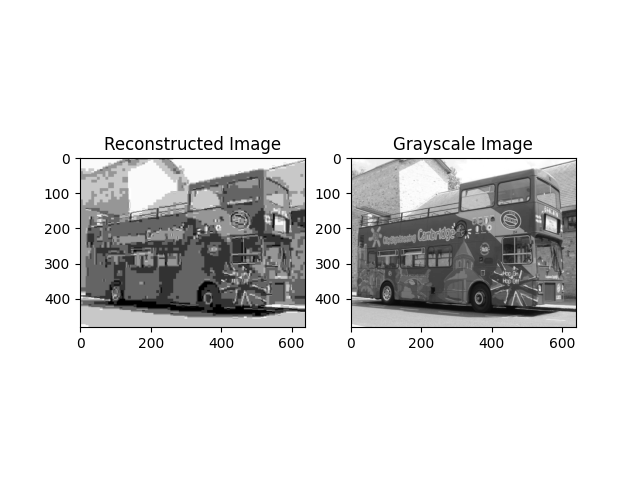
\includegraphics[width=0.7\textwidth]{../results/Quality: 2_comparison.png}
		\caption{Original and Reconstructed Image}
	\end{figure}
\end{frame}

\begin{frame}
	\frametitle{Quality Comparison}
	Here is the comparison of the reconstucted and the original image for a quality factor of 10:
	\begin{figure}
		\centering
		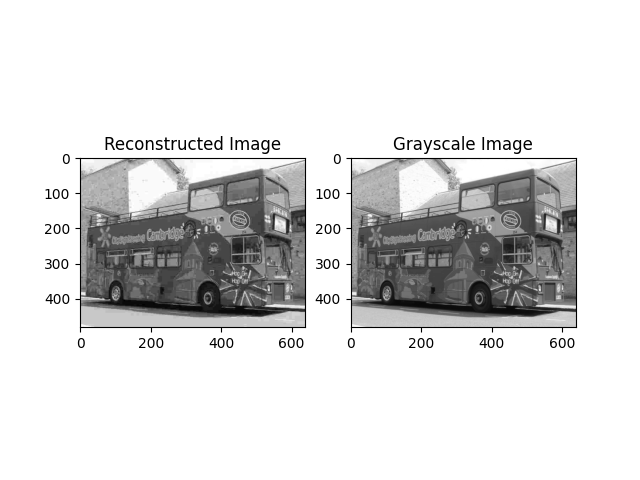
\includegraphics[width=0.7\textwidth]{../results/Quality: 10_comparison.png}
		\caption{Original and Reconstructed Image}
	\end{figure}
\end{frame}

\begin{frame}
	\frametitle{Quality Comparison}
	Here is the comparison of the reconstucted and the original image for a quality factor of 50:
	\begin{figure}
		\centering
		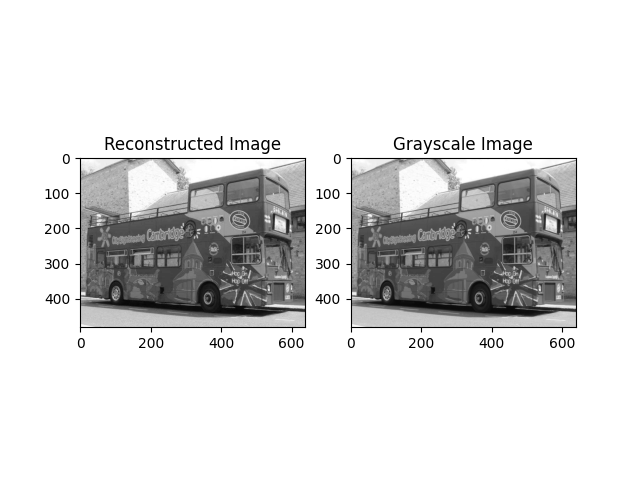
\includegraphics[width=0.7\textwidth]{../results/Quality: 50_comparison.png}
		\caption{Original and Reconstructed Image}
	\end{figure}
\end{frame}

\begin{frame}
	\frametitle{Quality Comparison}
	Here is the comparison of the reconstucted and the original image for a quality factor of 80:
	\begin{figure}
		\centering
		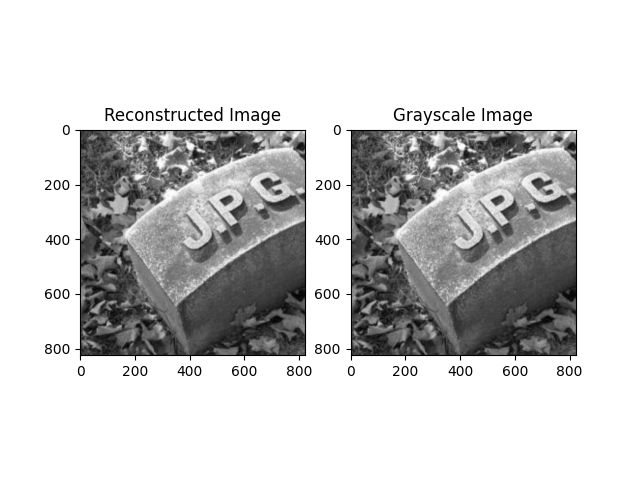
\includegraphics[width=0.7\textwidth]{../results/Quality: 80_comparison.png}
		\caption{Original and Reconstructed Image}
	\end{figure}
\end{frame}

\begin{frame}
	\frametitle{RMSE vs BPP}
	For the basic implementation, we have used the dataset from the miscellaneous category of the msrcorid dataset. We picked random 20 images and used 20 quality factors (in the range of 1 to 100) to plot the RMSE vs BPP graph. Here is the graph:

	\begin{figure}
		\centering
		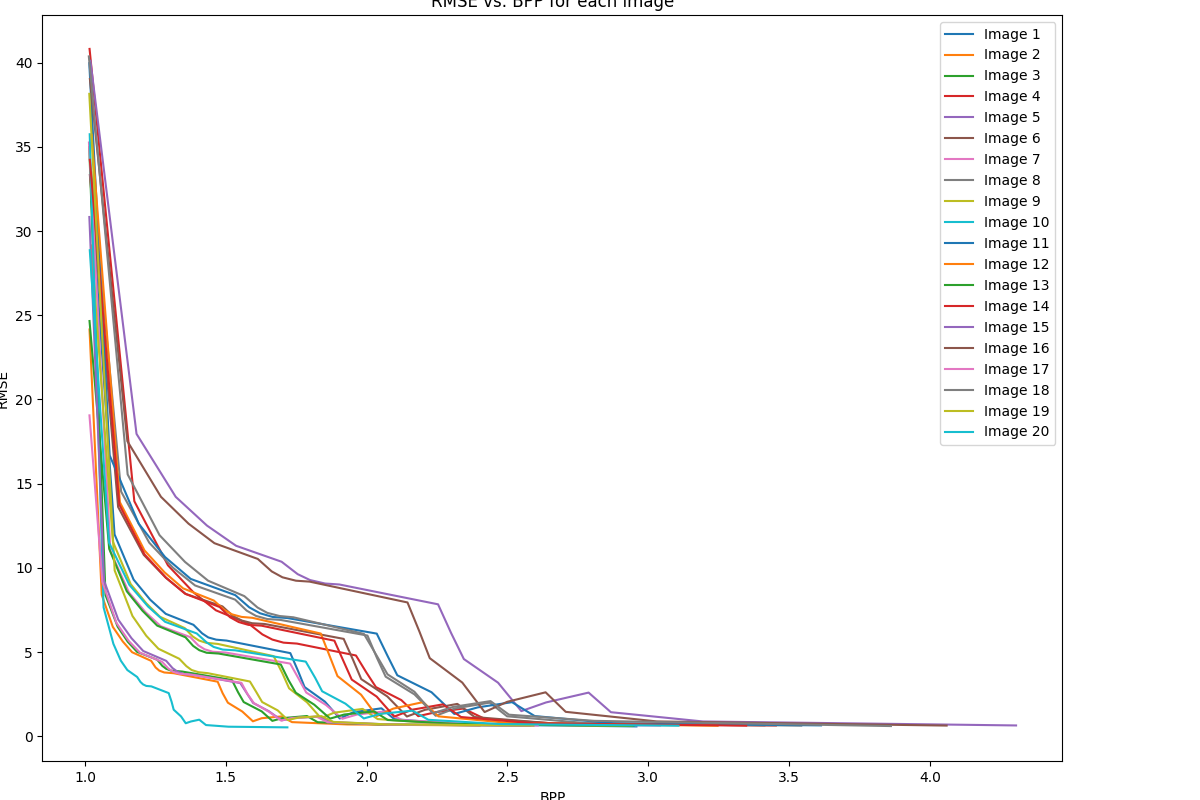
\includegraphics[width=0.7\textwidth]{../results/basic.png}
		\caption{RMSE vs BPP}
	\end{figure}
	
\end{frame}

\begin{frame}
	\frametitle{Comparison of Basic vs JPEG}
	The following plot shows how the basic algorithm performs as compared to the JPEG algorithm. 
	
	\begin{figure}
		\centering
		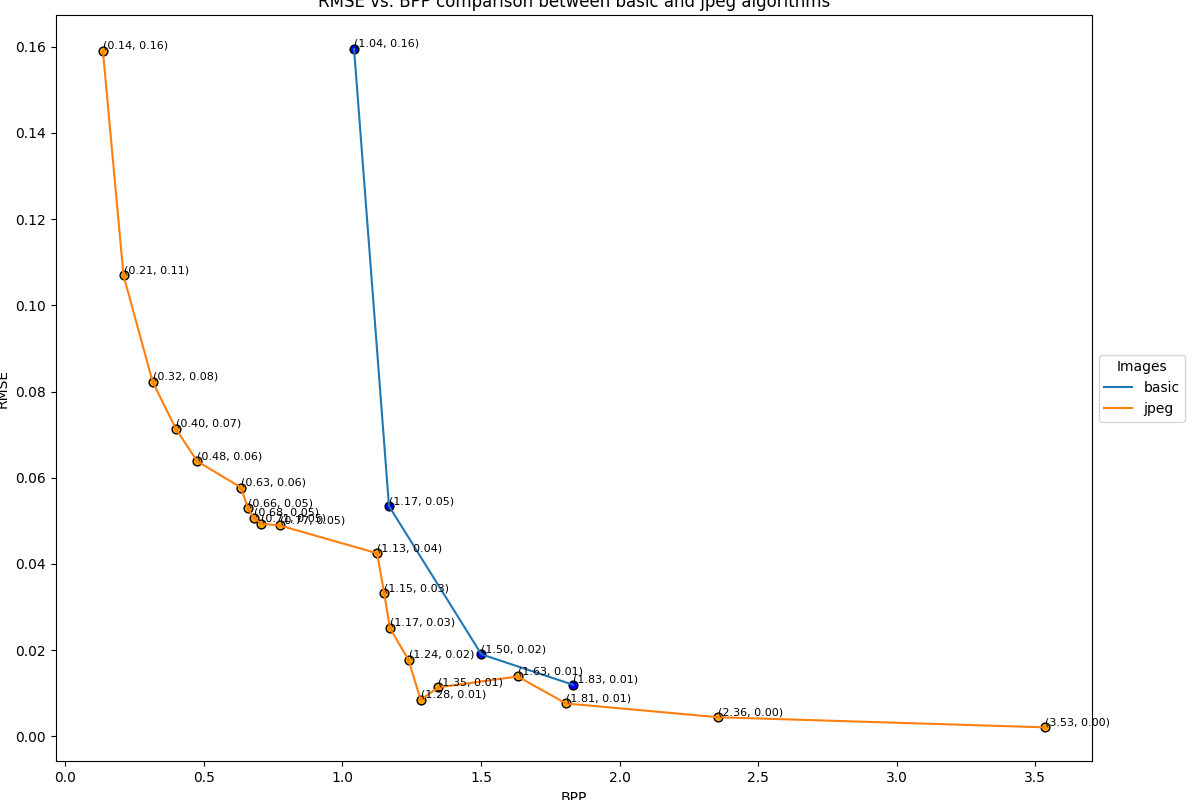
\includegraphics[width=0.7\textwidth]{../results/basic_jpeg_comparison.png}
		\caption{Comparison of Basic and JPEG}
	\end{figure}
\end{frame}

\section{Run Length Encoding}

\begin{frame}
	\frametitle{Run Length Encoding}
	The quantized DCT coefficients are arranged in a zigzag order. This pattern leaves a bunch of consecutive zeros at the end.

	\vspace{1cm}

	In runlength encoding, we replace the consecutive zeros with a pair of numbers: the number of zeros and the value of the next non-zero element. This reduces the size of the data to be stored.
\end{frame}

\begin{frame}{RMSE vs BPP}
	The dataset of images from the miscellaneous category of the msrcorid dataset was used to plot the RMSE vs BPP graph. Here is the graph:

	\begin{figure}
		\centering
		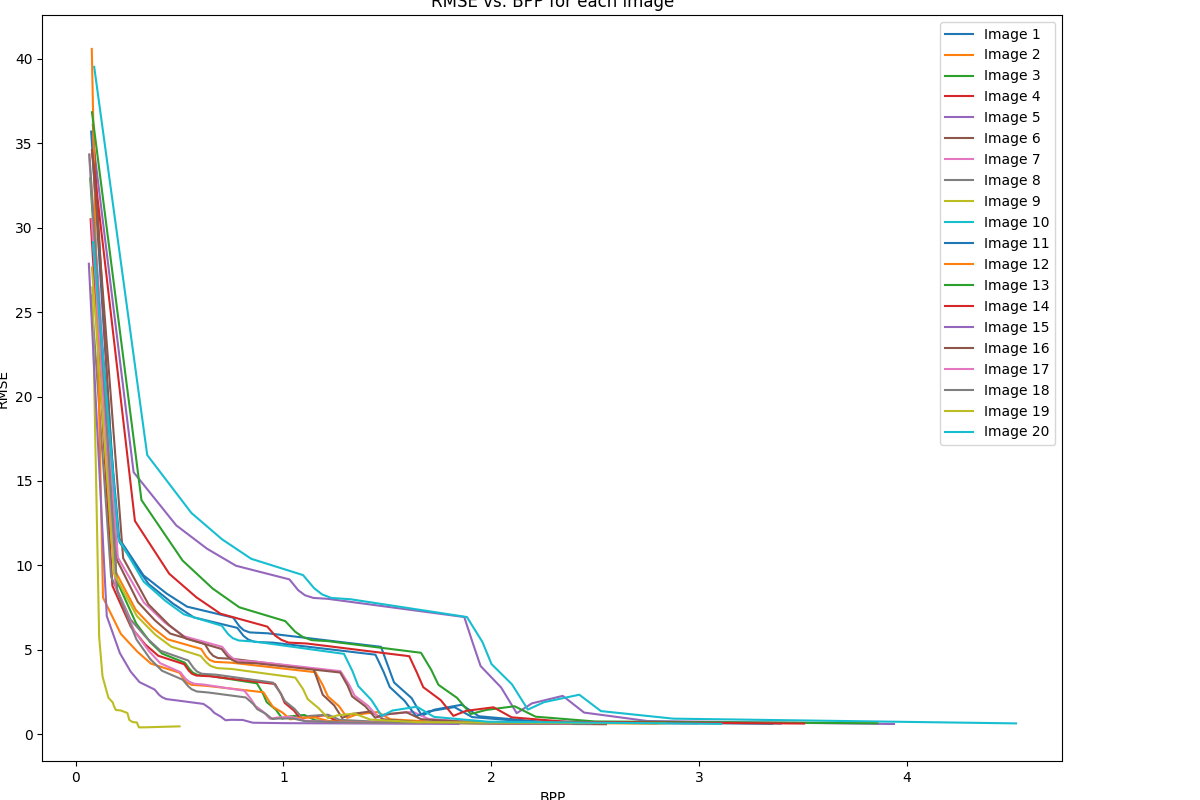
\includegraphics[width=0.7\textwidth]{../results/runlength.png}
		\caption{RMSE vs BPP}
	\end{figure}

\end{frame}

% \section{Comparison of Basic and Run Length Encoding}
\begin{frame}
	\frametitle{Comparison of Basic and Run Length Encoding}

	\begin{figure}
		\centering
		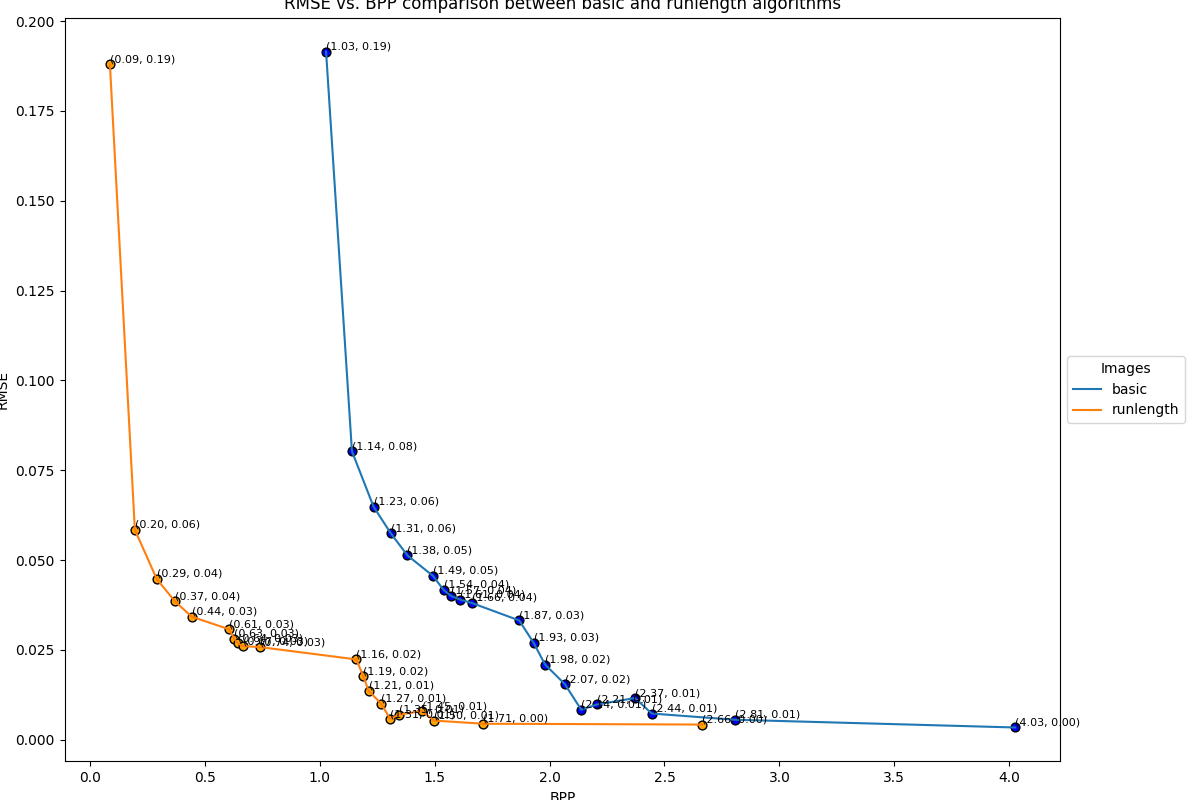
\includegraphics[width=0.7\textwidth]{../results/basic_runlength_comparison.png}
		\caption{Comparison of Basic and Run Length Encoding}
	\end{figure}
\end{frame}

\begin{frame}
	\frametitle{Comparison of Run Length Encoding and JPEG Algorithm}

	\begin{figure}
		\centering
		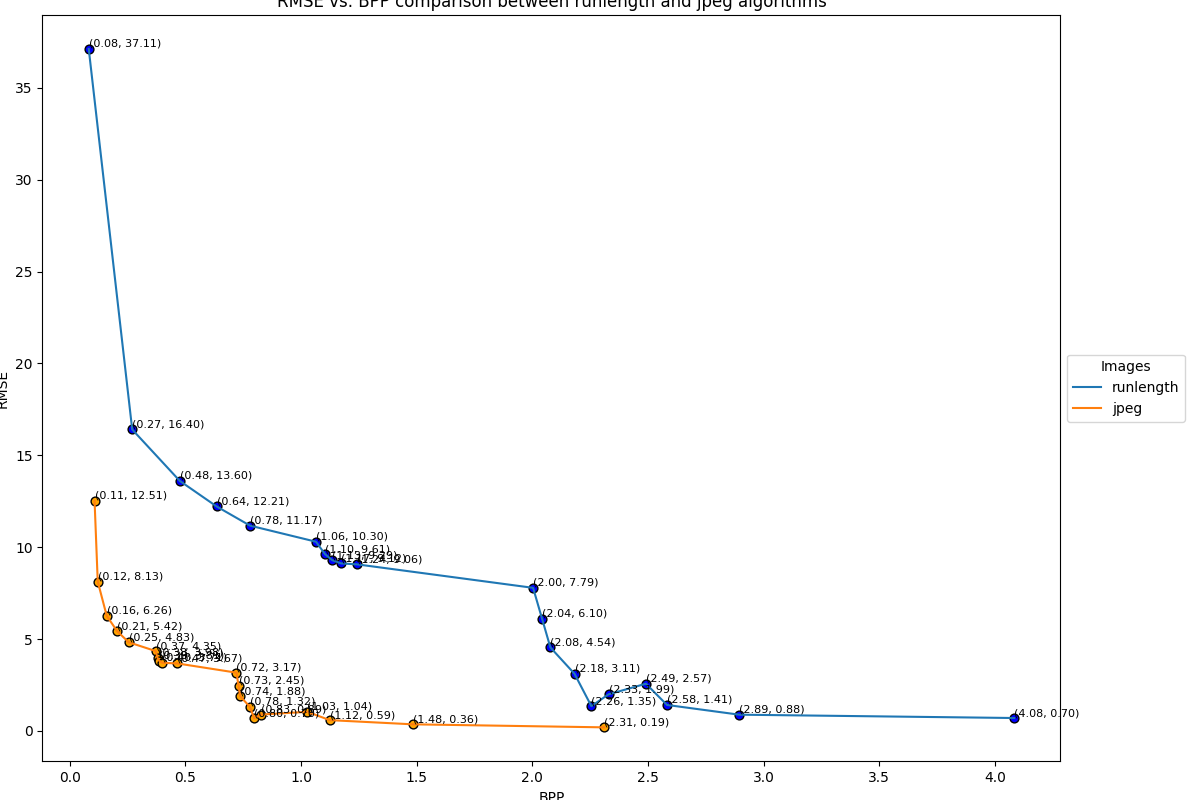
\includegraphics[width=0.7\textwidth]{../results/runlength_jpeg_comparison.png}
		\caption{Comparison of Basic and Run Length Encoding}
	\end{figure}
\end{frame}

\section{Coloured JPEG}

\begin{frame}
	\frametitle{Quality Comparison}
	Here is the comparison of the reconstucted and the original image for a quality factor of 10:
	\begin{figure}
		\centering
		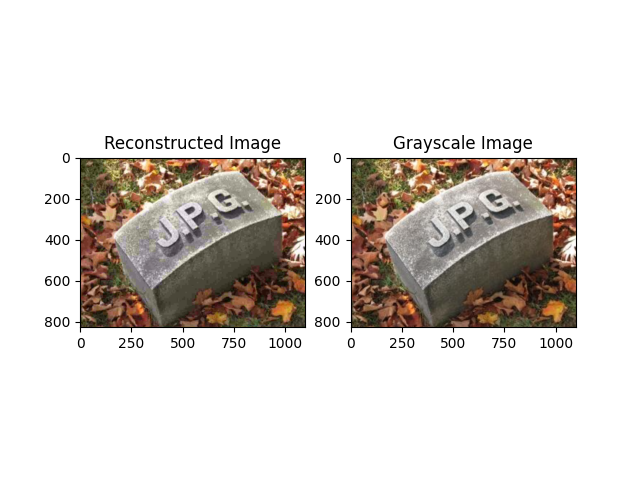
\includegraphics[width=0.7\textwidth]{../results/Quality: 10_comparison_colour.png}
		\caption{Original and Reconstructed Image}
	\end{figure}
\end{frame}


\begin{frame}
	\frametitle{Quality Comparison}
	Here is the comparison of the reconstucted and the original image for a quality factor of 80:
	\begin{figure}
		\centering
		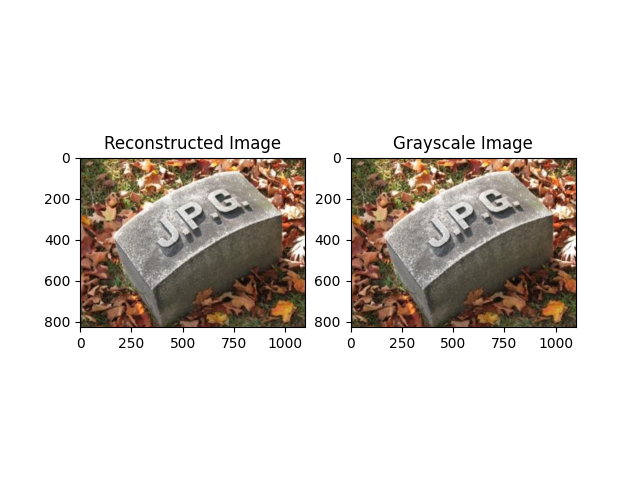
\includegraphics[width=0.7\textwidth]{../results/Quality: 80_comparison_colour.png}
		\caption{Original and Reconstructed Image}
	\end{figure}
\end{frame}
\section{Principal Component Analysis}

\begin{frame}
	\frametitle{PCA on a Single Grayscale Image}
	\begin{itemize}
		\item Pad the image suitably to make dimensions a multiple of $8$.
		\item Divide the image into patches of size $8 \times 8$ and flatten them into column vectors.
		\item Compute the column correlation and row correlation matrices of the matrix of flattened patches.
		\item Compute the kronecker product of the two matrices and extract eigenvectors of this matrix with the top $k$ eigenvalues. These eigenvectors are the principal components.
		\item Now project the original image onto the column space of these eigenvectors. The resulting matrix is the compressed image.
		\item Reconstruct the image by multiplying the compressed image with the transpose of the eigenvectors. 
	\end{itemize}
\end{frame}

\begin{frame}
	\frametitle{PCA on a Dataset of Grayscale Images}
	\begin{itemize}
		\item Pad the images suitably to make dimensions a multiple of $8$.
		\item Divide each image into patches of size $8 \times 8$ and flatten them into column vectors. Create a matrix whose columns are the flattened image patches.
		\item Compute the column correlation and row correlation matrices of the matrix of flattened patches.
		\item Compute the kronecker product of the two matrices and extract eigenvectors of this matrix with the top $k$ eigenvalues. These eigenvectors are the principal components.
		\item Now project each of the original images onto the column space of these eigenvectors. The resulting matrix is the compressed image.
		\item Reconstruct any image by multiplying the compressed image with the transpose of the eigenvectors. 
	\end{itemize}
\end{frame}

\begin{frame}
	\frametitle{PCA on a Single Coloured Image}
	\begin{itemize}
		\item Pad the image the suitably to make dimensions a multiple of $8$.
		\item Treat each image channel as a grayscale image and run the PCA algorithm on each channel separately.
		\item Extract the compressed image for each channel separately and merge them to get the compressed coloured image.
		\item Reconstruct the image by multiplying the compressed image of each channel with the transpose of the eigenvectors of that channel.
		\item Merge the reconstructed channels to get the reconstructed coloured image.
	\end{itemize}
\end{frame}

\begin{frame}
	\frametitle{PCA Results}
	\begin{figure}
		\centering
		% \includegraphics{}
		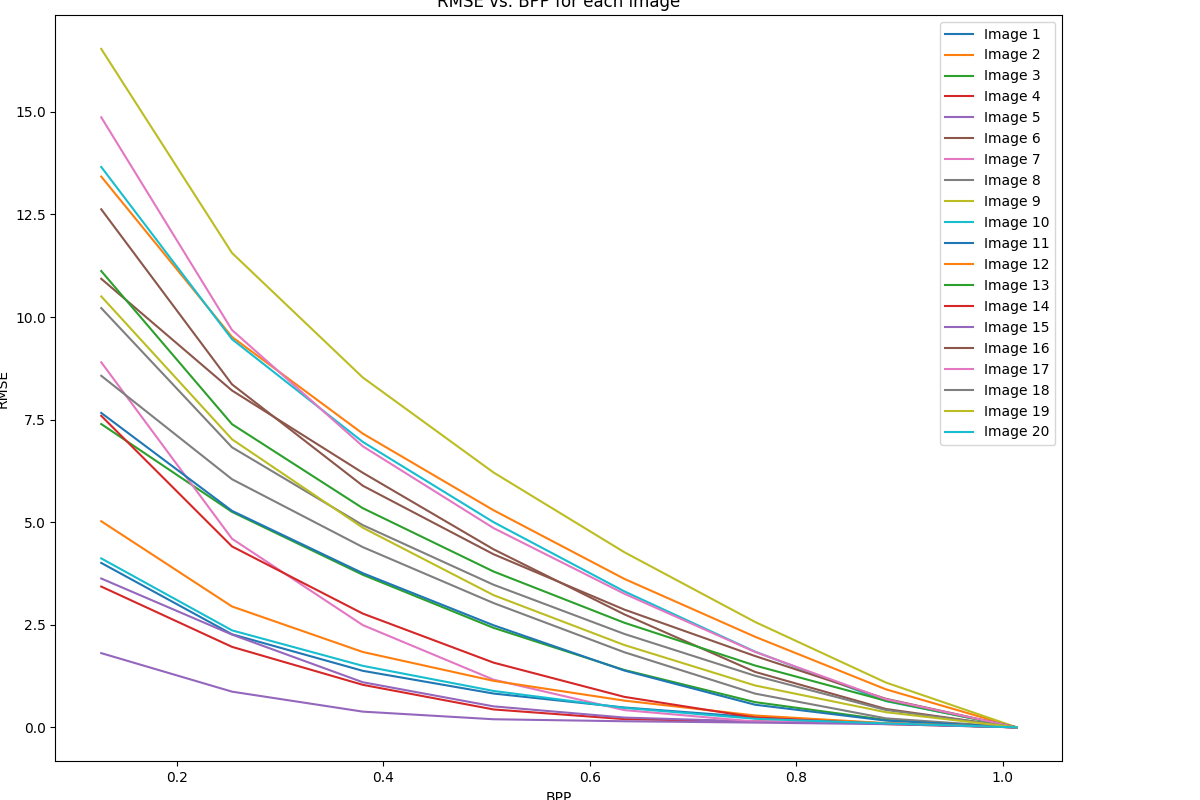
\includegraphics[width=0.7\textwidth]{../results/pca.png}
		\caption{RRMSE vs BPP for PCA on a grayscale image}
	\end{figure}
\end{frame}

\begin{frame}
	\frametitle{PCA Results}
	\begin{figure}
		\centering
		% \includegraphics{}
		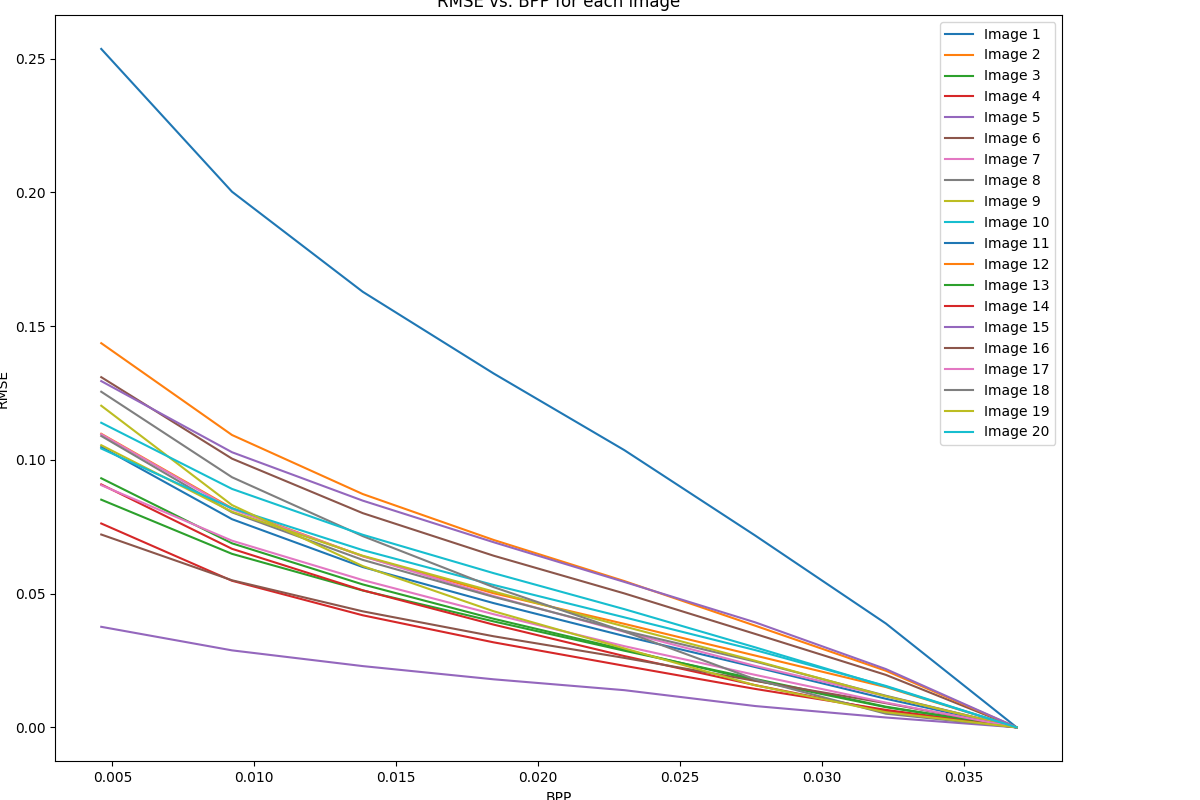
\includegraphics[width=0.7\textwidth]{../results/dpca.png}
		\caption{RRMSE vs BPP for PCA on a dataset of grayscale images}
	\end{figure}
\end{frame}

\begin{frame}
	\frametitle{PCA Results}
	\begin{figure}
		\centering
		% \includegraphics{}
		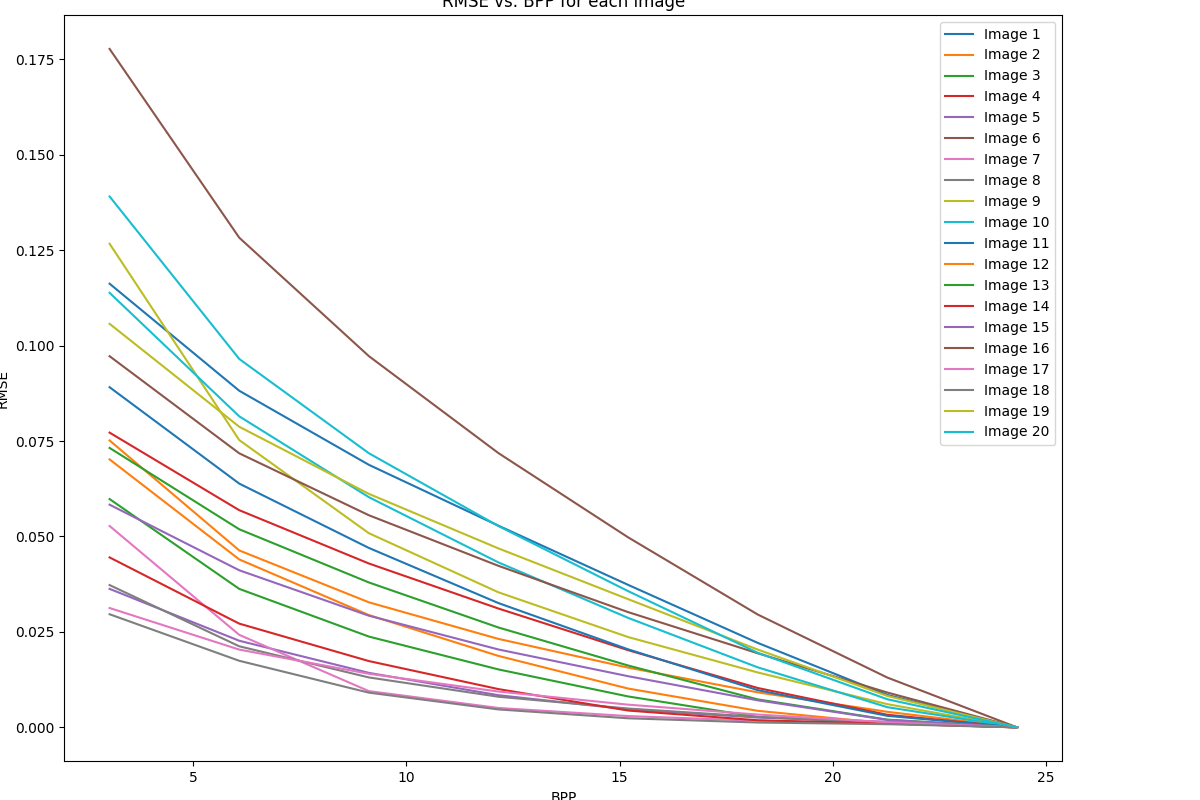
\includegraphics[width=0.7\textwidth]{../results/cpca.png}
		\caption{RRMSE vs BPP for PCA on a coloured image}
	\end{figure}
\end{frame}



\section{Paper Implementation}
\begin{frame}
    \centering
    {\Huge \textbf{Edge-Based Image Compression}}

	\vspace{1cm}
	This paper is based on the fact that edges contain semantically important information in an image. They present a lossy compression method for cartoon-like images.
\end{frame}

\begin{frame}
	\frametitle{Encoding Steps}
	\begin{itemize}
		\item Firstly, we need to detect edges in the image. The paper proposes Marr-Hildreth edge detector. However, based on our initial experiments, we found that the Canny edge detector works better.
		\item Now we store the result of edge detection using JBIG(Joint Bi-level Image Experts Group) encoding.
		\item Then, we encode the contour pixel values. Basically, we store the
		values from both sides of the edge. The extracted pixel values can be uniformly quantised to $2^q$ different values,
		where $q \in \{1, 2, \dots, 8\}$. Another parameter $d$, ensures that only every $d^{th}$ value along an edge is stored.
		\item The quantised and subsampled pixel value signal is then compressed by a PAQ compression method (lossless compression archiver).
		\item Now, we need to store the encoded data along with all the values of the hyper-parameters.
	\end{itemize}
\end{frame}

\begin{frame}
	\frametitle{Decoding Steps}
	\begin{itemize}
		\item We split our encoded file into the JBIG data and PAQ data part. 
		\item Both parts are then decoded by using the JBIG and the PAQ
		method, respectively.
		\item We reconstruct the quantised colours obtained by the PAQ part. The pixel values between the sampled points are computed by using linear interpolation along each edge.
		\item The JBIG data provides a bi-level edge image of the original image size. Given the image size and the edge pixel positions, the pixel values are arranged around the edges in the same order in which they have been encoded.
		\item Now, we have decoded the edge locations and the pixel values surrounding the edges. We use diffusion based inpainting to fill the remaining values.
	\end{itemize}
\end{frame}

\begin{frame}
	\frametitle{Results}
	\begin{figure}
		\centering
		% \includegraphics{}
		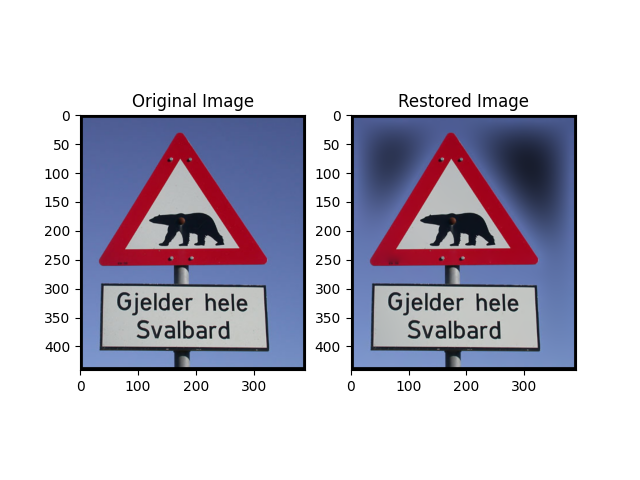
\includegraphics[width=0.7\textwidth]{../results/try_11_0.png}
		\caption{Original vs Reconstructed Image}
	\end{figure}
\end{frame}


\begin{frame}
	\frametitle{Results}
	\begin{figure}
		\centering
		% \includegraphics{}
		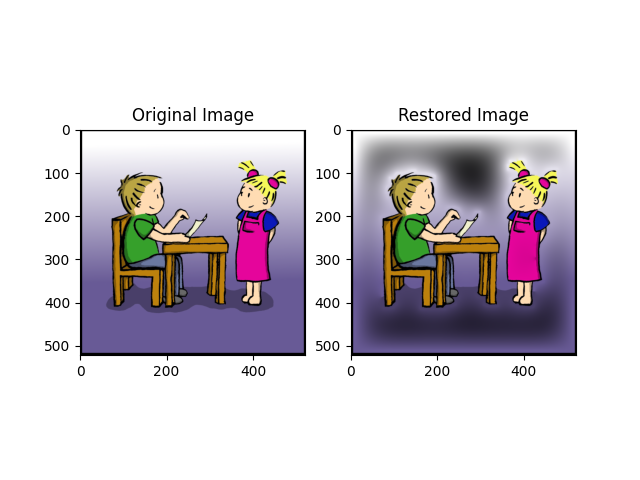
\includegraphics[width=0.6\textwidth]{../results/try_11_1.png}
		\caption{Original vs Reconstructed Image}
	\end{figure}
	To reduce the black patches in regions of the uniform intensity, we propose artificial segmentation of the image, and then handling the small segments normally.
\end{frame}


\begin{frame}
	\frametitle{Results}
	\begin{figure}
		\centering
		% \includegraphics{}
		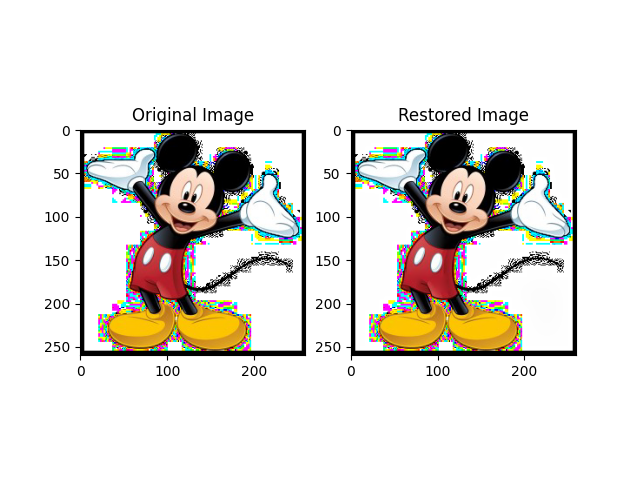
\includegraphics[width=0.7\textwidth]{../results/try_11_2.png}
		\caption{Original vs Reconstructed Image}
	\end{figure}
\end{frame}


\begin{frame}
	\frametitle{Results}
	\begin{figure}
		\centering
		% \includegraphics{}
		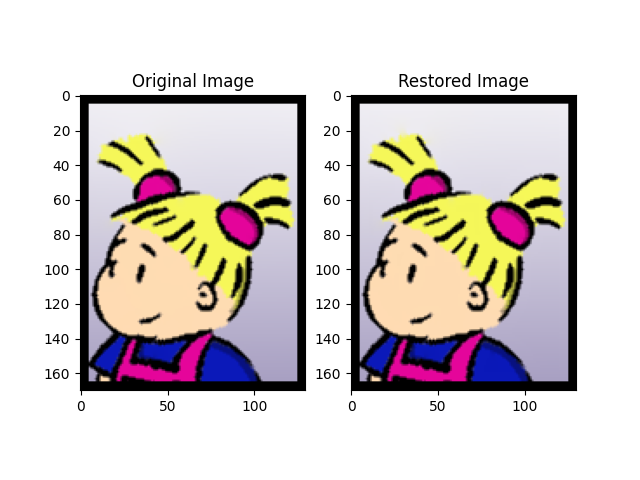
\includegraphics[width=0.7\textwidth]{../results/try_11_3.png}
		\caption{Original vs Reconstructed Image}
	\end{figure}
\end{frame}


\begin{frame}
	\frametitle{Results}
	\begin{figure}
		\centering
		% \includegraphics{}
		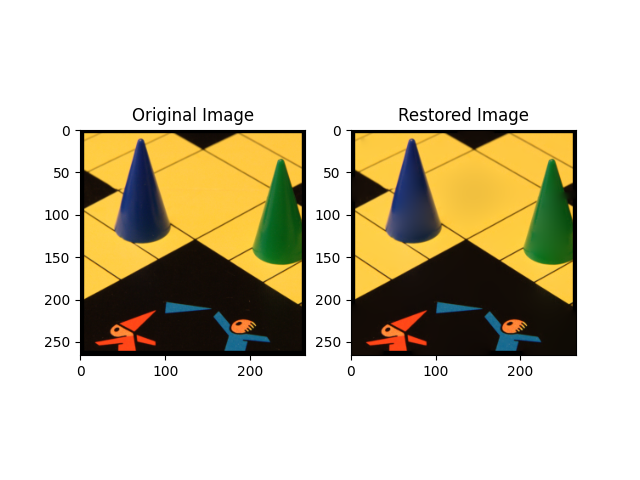
\includegraphics[width=0.7\textwidth]{../results/try_11_4.png}
		\caption{Original vs Reconstructed Image}
	\end{figure}
\end{frame}

\begin{frame}
	\frametitle{Results}
	\begin{figure}
		\centering
		% \includegraphics{}
		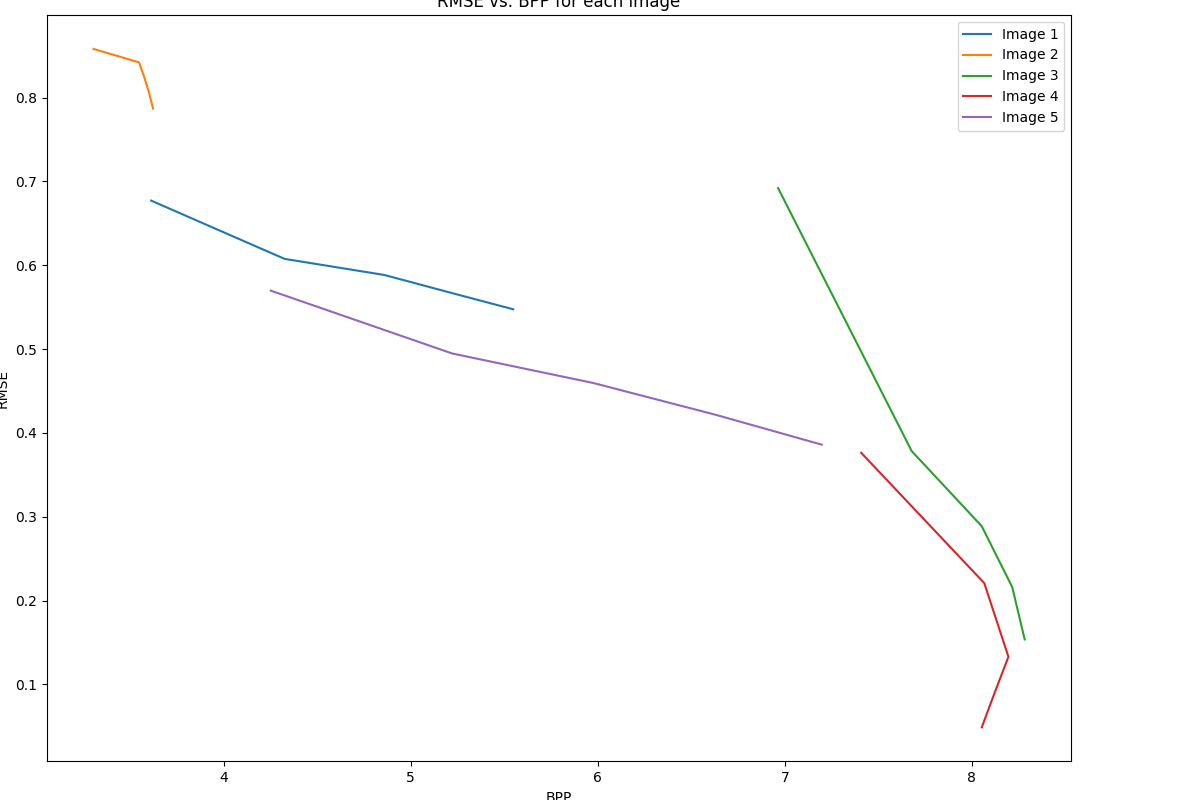
\includegraphics[width=0.7\textwidth]{../results/paper.png}
		\caption{Original vs Reconstructed Image}
	\end{figure}
\end{frame}




\section{Individual Contributions}

\begin{frame}
	\frametitle{Individual Contributions}
	\begin{alertblock}{Saksham Rathi}
		Basic Implementation\\
		Paper understanding and implementation\\
		Code Modularity\\
		Report Completion
	\end{alertblock}
	\begin{alertblock}{Kavya Gupta}
		Basic Implementation\\
		Coloured JPEG\\
		Paper understanding and implementation
	\end{alertblock}
	\begin{alertblock}{Shravan Srinivasa Raghavan}
		PCA\\
		Paper understanding and implementation
	\end{alertblock}

\end{frame}

\section{Innovations Incorporated}

\begin{frame}
	\frametitle{Innovations Incorporated}
	\begin{itemize}
		\item Runlength encoding and zigzag ordering of DCT coefficients
		\item PCA for a single grayscale image, a dataset of grayscale images (optimized memory with no redundancies in saving the model), and a single coloured image
		\item Comparison over different quantization matrices
		\item JPEG Implementation for a coloured image
		\item Implementation of the paper ``Edge-Based Image Compression with Homogeneous Diffusion''
		\begin{itemize}
			\item To detect borders of the image, we padded with cells of zero intensity
			\item To reduce the black patches in regions of uniform intensity, we are changing the window size (tradeoff between size and accuracy)
			\item Varied diffusion time for getting the best output for the target images (tradeoff between time and accuracy)
		\end{itemize}
	\end{itemize}
\end{frame}


\section{References}

\begin{frame}
	\frametitle{References}
	\begin{itemize}
		\item \href{https://docs.google.com/presentation/d/1-8xCg7o8Vtc9ghJf6y1Nkq9-TV0qSNfX/edit?usp=sharing&ouid=115909013767952805958&rtpof=true&sd=true}{\textcolor{blue}{\underline{CS663: Image Compression Slides}}}
		\item Course Textbook: ``Digital Image Processing'' by Rafael C. Gonzalez and Richard Woods, 3rd edition
		\item Using partial differential equations (PDEs) for image compression: M. Mainberger and J.Weickert, "Edge-Based Image Compression with Homogeneous Diffusion", CAIP 2009
		\item Osman Gokhan Sezer, Onur G. Guleryuz and Yucel Altunbasak, ``Approximation and Compression With Sparse Orthonormal Transforms'', IEEE Transactions on Image Processing, 2015
		\item \href{https://github.com/jeremyfell/image-compression/blob/master/image-compression.py}{\textcolor{blue}{\underline{Sample Image Compression Code}}}
		\item \href{https://github.com/adl1995/edge-detectors/blob/master/marr-hildreth-edge.py}{\textcolor{blue}{\underline{Marr-Hildreth Edge Detector}}}
	\end{itemize}
\end{frame}

\end{document}


